\chapter{Ramping parameter under the random graph model} % (fold)
\label{cha:ramping_parameter_under_the_random_graph_model}

Previous work~\cite{Sindel:2009vd} provided a connection between the clustered structure of a graph and an interpretation of concentration risk.
The methodology presented by the authors considered the effects of removing edges with weight under a (varying) threshold, on the community structure of a fully connected obligor-correlation matrix.
In particular, by computing the variation of the component structure of the graph, the authors have shown how to analyse concrete credit portfolios and identify sets of strongly connect obligors.


This thesis builds upon the aforementioned model and aims at describing the expected behaviour of the ramping parameter model for theoretical graph generation models under a few simplifying assumptions.
In this chapter, we focus on the random graph model, a well understood theoretical graph model, described in more detail in Section~\ref{sec:random_graph_model}.

In particular, we attempt to describe the expected behaviour of the curve designed by~\cite{Sindel:2009vd}, assuming that we have large, idealized, portfolios generated under simplifying assumptions,
and according to random graph model that generates them.
This curve could be hypothetically be later used to derived a more neutral weight-curve (see Equation~\ref{eq:ramping_integral}) and more accurately compute the concentration risk.


\section{Ramping parameter under random graph model} % (fold)
\label{sec:ramping_parameter_under_random_graph_model}


In this Section, we make use of the properties of the random graph model in order to make predictions about the ramping parameter and the concentration risk.
Contrasting to the original work on the ramping parameter~\cite{Sindel:2009vd}, rather than computing the concentration risk of a particular portfolio, we wish to describe the behaviour of the family of portfolios drawn from a given distribution.
In order to do this, certain assumptions about the portfolios must be made.
In particular, we assume:
\begin{itemize}
	\item the portfolios to be large, i.e. we assume that $n \rightarrow \infty$, where $n$ is the number of obligors
	\item the exposure of each individual obligor is $\frac{1}{n}$, i.e. the exposure is uniformly distributed amongst all obligors
	\item the elements of the dependency matrix to be independent from each other
\end{itemize}

\begin{remark}The dependency to large $n$ allows the results for the random graph model to hold exactly.
In practice, however, even large portfolios will be finite and there will be some error. This error is here not analysed.
\end{remark}




\begin{definition}
\label{def:equivalence_aux} 
Let $\rho \in \R$, and the function $f_\rho$ so that
\begin{equation}
\label{eqn:function}
f_\rho: C \rightarrow A\\
\\
a_{ij} = \begin{cases} 1 & \text{if } c_{ij} > \rho \\
                       0 & \text{if } c_{ij} \le \rho \\
                       0 & \text{if } i = j
        \end{cases}
\end{equation}
Let $g$ the pdf and $G$ the cdf of each element $c_{ij}$ of $C$.

By defining $p = 1-G(\rho)$, we can write
$$
P( a_{ij} = 0 ) = P(c_{ij} \le \rho) = G(\rho) = 1-p
$$
and conversely
$$
P( a_{ij} = 1 ) = P(c_{ij} > \rho) = 1 - G(\rho) = p
$$
\end{definition}

In a first step we define the space of correlation matrices 
\begin{definition}
The space of correlation matrices $\mathcal{C}_{n\times n} = \left( C, \mathcal{F},  g_C \right)$ consists of all matrices where
\begin{itemize}
\item[-] $C \in \R^{n \times n}$, such that $c_{ij} = c_{ji}$, $c_{ii} = 0$, 
\item[-] $\mathcal{F}$ is the Borel $\sigma-$algebra on $C$,
\item[-] and all elements $c_{ij}$ are i.i.d. random variables with a probability distribution $g$.
\end{itemize}
\end{definition}

We want to identify matrices in $\mathcal{C}$ with adjacency matrices using a construction like the function \ref{eqn:function} defined above.
As the image of $f$ depends only on $G(\rho)$  this map is not injective; more precisely two matrices $C_1$ and $C_2$ are mapped to the the same matrix $A$ if for each pair $i\neq j$ of indices the equation  $G(\rho) = 1-p$ is satisfied.
We use this relation to define equivalence classes:

\begin{definition}
\label{def:equiv_correlation}
Two matrices $C_1$ and $C_2$ are equivalent if the following condition is satisfied:
\begin{equation}C_1\sim C_2\quad \Leftrightarrow \quad \forall i,j \,\ f_{\rho}(c^1_{ij}) = f_{\rho}(c^2_{ij})\,.\end{equation}
Then the space of equivalence classes is denoted by $\widetilde{C}_{n\times n}$. 
\end{definition}



\begin{theorem}{Equivalence to random graph model.}
\label{thm:equivalence_random_graph_model}
Consider the following probability spaces:
\begin{enumerate}
	\item the space of equivalence classes of correlation matrices $\widetilde{C}_{n\times n}$,
	\item the space of unweighted adjacency matrices $\mathcal{A}_{n\times n} = \left( A, 2^A, P_A \right)$,
	\item the space of random graphs $G_{n,p}$
\end{enumerate}
\noindent where,
\begin{itemize}
	\item[] $A \in \{0,1\}^{n \times n}$ such that $\forall i,j\,  a_{ij} = a_{ji} \text{ and } a_{ii} = 0$,
	\item[] $P_A = \begin{cases} 1 & \text{with probability } p,\\0 & \text{with probability } 1-p\end{cases}$,
	\item[] $P_C$ is some probability distribution,
	\item[] an adjacency matrix is a (0,1)-matrix with zeros on its diagonal.
\end{itemize}
The probability spaces are equivalent.
\end{theorem}

\begin{proof}

(2) $\Leftrightarrow$ (3):
Given that (i) a graph is defined unequivocally by its adjacency matrix, that (ii) all elements of $a_{ij}$ are by definition independent and that (iii) $P_A$ follows the same probability distribution as in $G_{n,p}$, both probability spaces are equivalent.
 % follows by the definition of $G_{n,p}$.
\\
(1) $\Leftrightarrow$ (2):
The equivalence of $\widetilde{\mathcal{C}}_{n\times n}$ and $\mathcal{A}_n$ is a direct consequence of the definition~\ref{def:equiv_correlation} of the equivalence classes \\
\end{proof}

\vspace{0.5cm}

By making an assumptions on the distribution of the portfolio interdependency or correlation matrix $\rmat$, theorem~\vref{thm:equivalence_random_graph} allows us to apply the results of the random graph model to the study of the ramping parameter.
The original work of~\cite{Sindel:2009vd} assumes the $\rij$ to non-negative correlation values in the interval $[0,1]$, and relies on the empirical distribution of the portfolio values.
% without making any expl assumptions on the distribution of the values.

In practice the matrix $\rmat$ can be generated by multiplying a set of (independent or correlated) risk factors with the dependencies of each obligor to these risk factors.
% \todo{example}
Alternatively, it could also be generated either by expert knowledge (in which case one would expect the matrix to be rather sparse), by a pure correlation of stock prices of the obligors, or even by a hybrid approach.

In light of this, no general assumptions can be made over the distribution of the values of $\rmat$ and we will be studying the behaviour of the ramping parameter under the following distributions:
(1) the uniform distribution, and a skewed distribution, (2) the truncated exponential distribution.

\subsection{Giant component} % (fold)
\label{sub:giant_component}

As seen in Section~\ref{sub:giant_component}, the giant component of the $G_{n,m}$ exists when $c \ge 1$, $c$ being the mean degree of $G$.
This means that a giant component is expected to exist when each vertex is in average connected to at least one other vertex.
As we have seen, the relative size $S$ of the giant component is given by:
\begin{equation}
	S = 1 + \frac{W(-c e^{-c})}{c},
\end{equation}
\noindent where $W$ is the Lambert-$W$ function.
Although there is no closed-form solution for this equation, it is possible to solve it numerically (e.g. by using the software package~\cite{sympy}).

The largest connected component of the effective correlation matrix is essential to computing the ramping parameter.
Whenever it exists, the giant component is therefore relevant.

We note that, under theorem~\ref{thm:equivalence_random_graph_model}, the mean degree $c$ is connected to the distribution of the values of the correlation matrix by its c.d.f..
In fact, $c = p (n-1)$, which as we defined in~\ref{def:equivalence_aux} can be rewritten as $c = (1-G(\rho)) (n-1)$, where $G$ is the c.d.f. of the elements of the correlation matrix.


\subsubsection{Uniform distribution of obligor correlations} % (fold)
\label{ssub:uniform_distribution}

By assuming that the $\rij \sim  U(0,1)$, the c.d.f. is trivially $G(\rho) = \rho$, and therefore $c = (1 -\rho)(n-1)$.
As we will see, the giant component therefore appears at a very early stage in the evolution of the ramping parameter, and so the community structure will be largely dominated by it, which can be seen in Figure~\vref{fig:uniform_giant_component}.
\begin{figure}[tb]
	\centering
	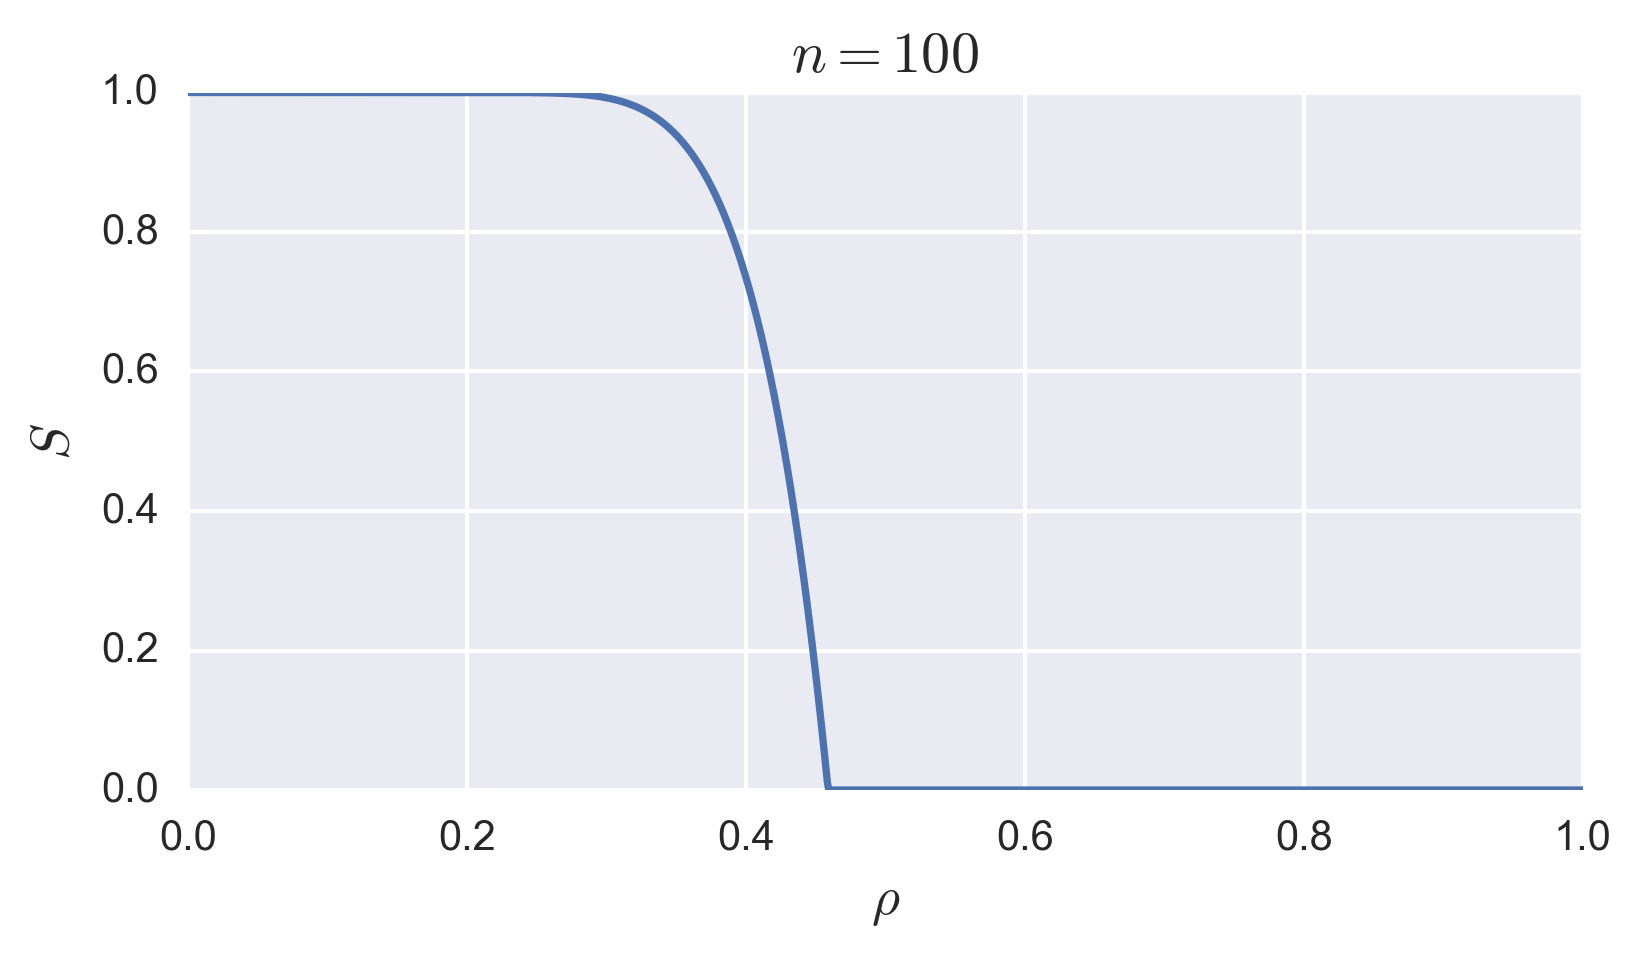
\includegraphics[scale=.8]{figures/3_uniform_giant_component.png}
	\caption{Relative size $S$ of giant component as a function of the ramping parameter $\rho$ given an uniform distribution of the correlation weights.}
	\label{fig:uniform_giant_component}
\end{figure}

% subsubsection uniform_distribution (end)

\subsubsection{Truncated exponential distribution} % (fold)
\label{ssub:truncated_exponential_distribution}

As we have seen in Section~\ref{ssub:uniform_distribution}, the giant component clearly dominates the community structure of the graph for the most values of the ramping parameter.
In a real world portfolio, it is likely that most correlations will be near zero, and that the latent structure of the inter-obligor matrix is revealed by a small set of strong interconnections.

In order to represent this, we assume that the $\rij$ are distributed according to the truncated exponential distribution.
The distribution is similar to the exponential distribution, but it is restricted to the domain $[0,1]$.
Like the exponential distribution, it is governed by one parameter: $\alpha$.
Its p.d.f. is as follows
\begin{equation}
	g(x) = - \frac{\alpha e^{- \alpha x}}{1-e^{-\alpha}}
\end{equation}
\noindent and the c.d.f. given by
\begin{equation}
	G(x) = \frac{1 - e^{-\alpha x}}{1-e^{-\alpha}}.
\end{equation}
The behaviour of the p.d.f. can be seen in figure~\vref{fig:exponential_distribution}. Larger values of the parameter $\alpha$ lead to more probability being concentrated with lower values of the r.v..
\begin{figure}[tb]
	\centering
	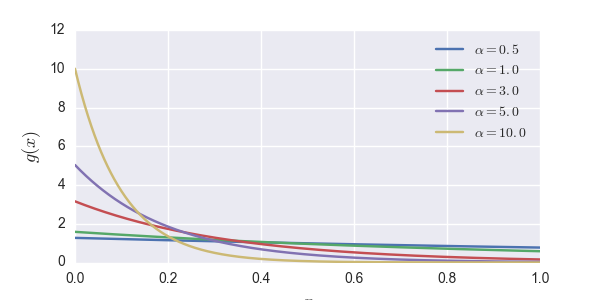
\includegraphics[scale=.8]{figures/3_exponential_distribution_pdf.png}}
	\caption{Probability density function of truncated exponential distribution with different values of the parameter $\alpha$.}
	\label{fig:exponential_distribution}
\end{figure}
The fact that much more probability density is concentrated on lower correlation values leads to an earlier and smoother disaggregation of the giant component.
The point at which the giant component disappears is also strongly dependent on the value of the parameter $\alpha$, which can be observed in figure~\vref{fig:exponential_giant_component}.
\begin{figure}[tb]
	\centering
	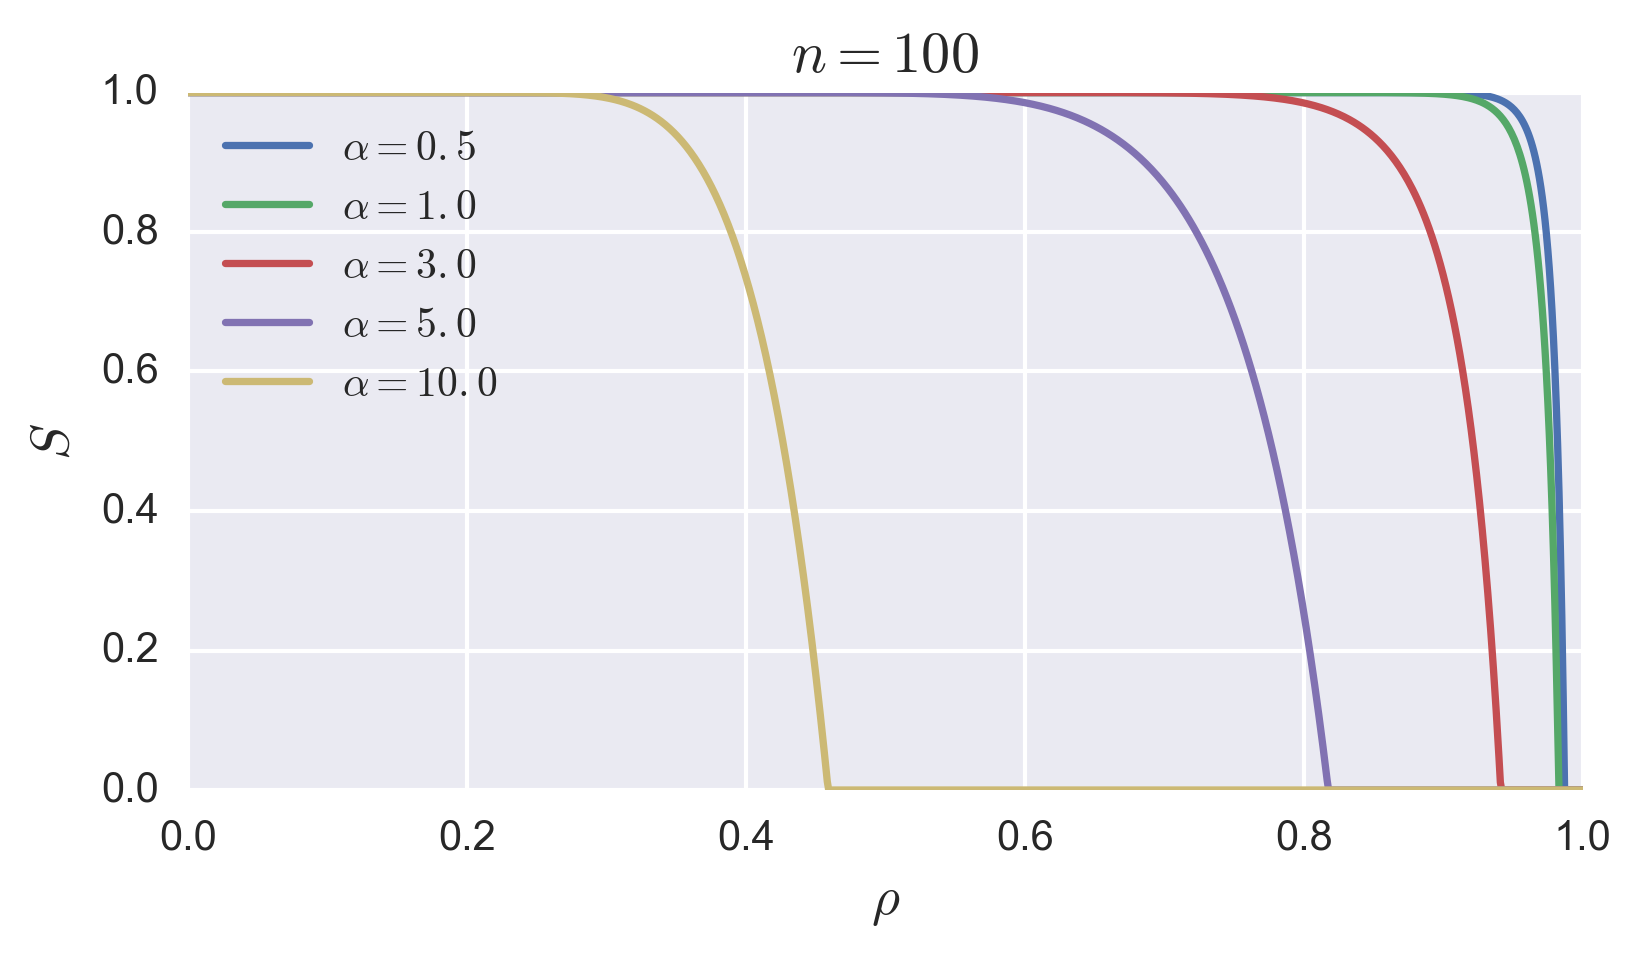
\includegraphics[scale=.8]{figures/3_exponential_giant_component.png}
	\caption{Relative size $S$ of giant component as a function of the ramping parameter $\rho$ given truncated exponential distributions  of the correlation weights with different parameters $\alpha$.}
	\label{fig:exponential_giant_component}
\end{figure}
This is already of great interest to the study of the ramping parameter, since it indicates a strong sensitivity to the distribution of the correlation values, independently of whether additional structure being available (which goes beyond of this chapter).

% subsubsection uniform_distribution (end)



% subsection giant_component (end)

\subsection{Small components' sizes} % (fold)
\label{sub:small_component_sizes}

% Using the random graph model we know 
From the previous chapter, we know that in the random graph model, the probability distribution of $\pi_s$, i.e. the probability that a randomly chosen node in the graph belongs to a component of size $s$.
We also know that this distribution complements the giant component
\begin{equation}
	\sum_{s=1}^{\infty} \pi_s = 1 - S
\end{equation}
\noindent and that it is given by
\begin{equation}
\label{eq:dist_size_components}
	\pi_s = \frac{1}{s!}\left[  \frac{d^{s-1}}{dh^{s-1}}e^{s c(h-1)}  \right] = \frac{e^{-s c} (s c)^{s-1}}{s!},
\end{equation}
What we are interested is, however, the actual number of components with size $s$.
This can be easily derived by considering that $n_s$ will be related to $\pi_s$ in that $s$ nodes will belong to a component of size $s$.
Therefore, 
\begin{equation}
	n_s = \frac{\pi_s}{s} = \frac{e^{-s c} (s c)^{s-1}}{s\,s!}.
	\label{eq:n_s}
\end{equation}
As hinted above, the situation is clearly dependent on whether the giant component exists in the graph.
In order to illustrate this, we show a histogram of the distribution of $n_s$ in figure~\ref{fig:distribution_sizes}.
\begin{figure}[tb]
	\centering
	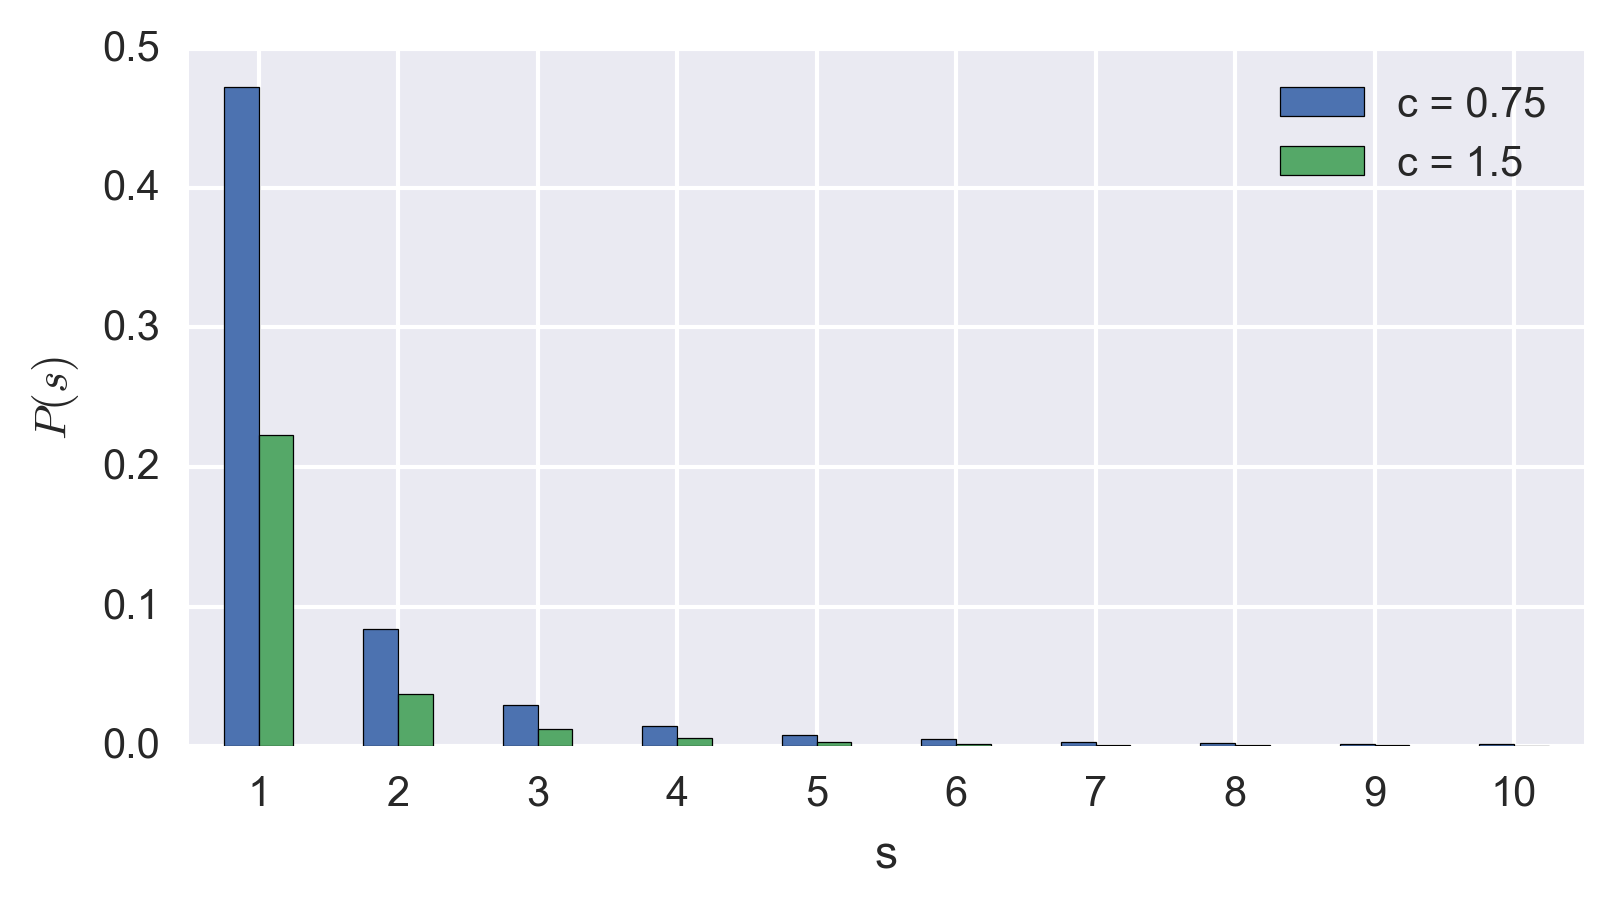
\includegraphics[scale=.9]{figures/3_distribution_sizes.png}}
	\caption[Histogram of $n_s$ for graphs with two different mean degree values.]{Histogram of $n_s$ for graphs with two different mean degree values. $c=0.75$ means that there is no giant component while $c=1.5$ guarantees the presence of the giant component. As can be seen, the probabilities of the component sizes is significantly lower in the case where the giant component exists, the reason for this being the fact that a fraction of the nodes belongs to the giant component and not to a small component.}
	\label{fig:distribution_sizes}
\end{figure}


\begin{theorem}{Size of the largest component.}
\label{thm:max_comp_size}
Let $n_s$ be the distribution of the non-giant component sizes under the random graph model, $k$ be the number of components in the graph, $C_i$ the size of component $i$.
Then $Y=max\left\{ C_1,\ldots,C_k\right\}$, the size of the largest non-giant component in the network, is a r.v. with probability distribution given by
$F_Y(y) = (\sum_{s=1}^{y} n_s)^k$.
\end{theorem}
\begin{proof}
Since every edge in the network exists independently, the $C_i$ variables are i.i.d. with p.d.f. given by equation~\ref{eq:n_s}.
We know that 
$$P(Y\le y) = P (C_1 \le y, \ldots , C_k \le y) = \Pi_{i=1}^{k} P(C_i \le y)$$
By definition, $P(C_i \le x) = \sum_{s=1}^y n_s$, and so $F_Y(y) = \left( \sum_{s=1}^y n_s \right)^k$.
\end{proof}
\vspace{0.3cm}
\begin{remark}
Theorem~\vref{thm:max_comp_size} is only of limited help due to the fact that the number of components $k$ in the graph is not known a priori in the random graph model.
Its distribution is, however, known and can be used to compute a numerical estimate of the distribution above.
\end{remark}

If we consider $c > 1$, then the size of the largest component is trivially given by $S$.
In the case of $c \le 1$, then we must consider the distribution $Y$ given by Theorem~\ref{thm:max_comp_size}.
We consider the expected number of components to be given by
\begin{equation}
	k = \sum_{s=1}^{\infty} n_s
\end{equation}
which can be seen in Figure~\ref{fig:gnp_number_components}.


And finally, the expected maximal component size is simply given by the definition of the expected value.
\begin{equation}
	E[Y] = \sum_s s P(Y=s)
	\label{eq:e_y}
\end{equation}
and can be seen in Figure~\ref{fig:gnp_largest_component} for all values of  the parameter $\rho$ in different truncated exponential probabilities.

\begin{figure}[hb]
	\centering
	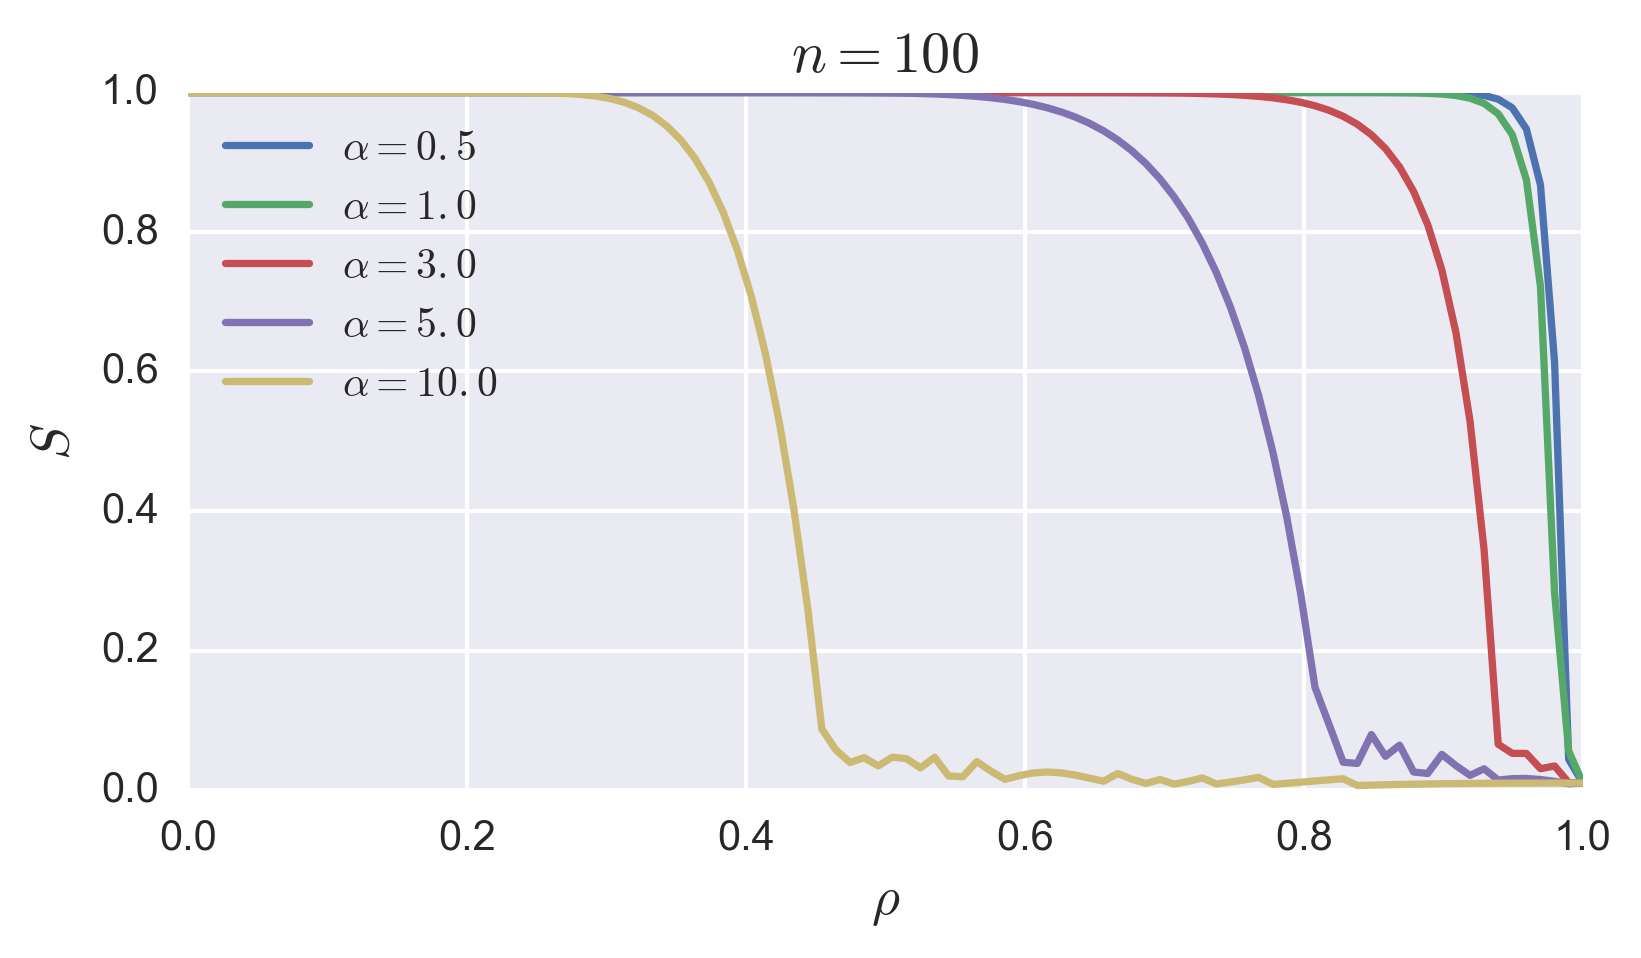
\includegraphics[scale=0.9]{figures/3_largest_component.png}
	\caption[Expected relative size of the largest component.]{Expected relative size of the largest component. One can see the result of some numerical instability in the region near the phase transition. The reason behind this instability is still unknown.}
	\label{fig:gnp_largest_component}
\end{figure}



\begin{theorem}{Expected ramping parameter value.}
	Let $Y$ be the size of the largest small component in a random graph, and $S$ the relative size of the giant component.
	Let $Pf$ be a uniformly exposed portfolio with correlation matrix $C$ whose elements are independently distributed according to the cdf $G$.
	Then, the expected ramping parameter value for $Pf$ and $\ramp$ by
	$$\max\left\{\frac{E[Y]}{n}, S\right\}$$
	is given by $c$.
\end{theorem}
\begin{proof}
	The largest component is either the the giant component (if it not exists, $S=0$) or the largest small component, with expected value given by Equation~\ref{eq:e_y}.
	Because the exposures are uniformly distributed across obligors, $EAD_j = 1/n$, the value of
	$$R(\ramp) = \max_{C_k} \left(  \frac{\sum_{j\in C_k} \textrm{EAD}_j}{\sum_i \textrm{EAD}_i}  \right)$ 
	\noindent reduces trivially to 
	$$R(\ramp) = \max_{C_k} \left(  \frac{\sum_{j\in C_k} 1/n}{\sum_i 1/n}  \right) = \max_{C_k} \frac{\sum_{j\in C_k} 1}{n}$$
	and therefore
	$$E[R(\ramp)] = \max\left\{\frac{E[Y]}{n}, S\right\}
\end{proof}

\noindent An example of the curve defined by this value can be seen in Figure~\ref{fig:gnp_largest_component} above.
The usefulness of this result is discussed in the following Section.



\begin{figure}[hb]
	\centering
	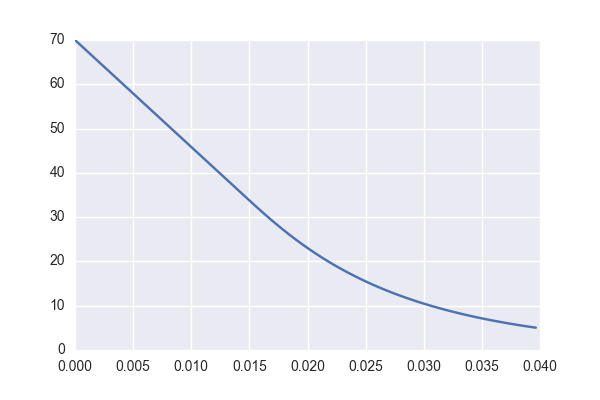
\includegraphics[scale=0.8]{figures/gnp_number_components.png}
	\caption{Expected number of components as a function of the probability $p$ of the $G(n,p)$ model.}
	\label{fig:gnp_number_components}
\end{figure}
% subsection component_sizes (end)







% \begin{itemize}
% 	\item The variation of the ramping parameter is equivalent to having random graphs generated with different $p$ probabilities.
% \end{itemize}


% section ramping_parameter_under_random_graph_model (end)

% chapter ramping_parameter_under_the_random_graph_model (end)